\documentclass[a4paper]{article}
\usepackage[pdftex]{graphicx}
\usepackage[utf8]{inputenc}
\usepackage{enumerate}
\usepackage{siunitx}
\usepackage{colortbl}
\usepackage{tikz}
\usepackage{href-ul}
\hypersetup{
	colorlinks=true,
	linkcolor=blue,
	urlcolor=blue}
\sisetup{locale=DE} 
\usepackage{icomma}
\usepackage{amssymb}
\usepackage{geometry}
\geometry{a4paper, top=15mm, left=15mm, right=15mm, bottom=15mm,
	headsep=10mm, footskip=12mm}

\begin{document}
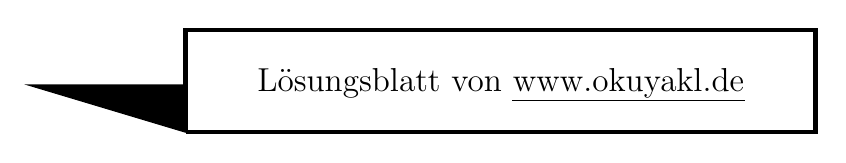
\begin{tikzpicture}(10,3)
	\draw[ultra thick](2,0) --(10,0) -- (10,1.3) --(2,1.3) -- (2,0);
	\draw[fill=black](2,0)-- (0,.6) -- (2,.6) -- (2,0);
	\node at (6,.6) {\large Lösungsblatt von \href{https://www.okuyakl.de}{www.okuyakl.de}};
\end{tikzpicture}
\vspace{0.5 cm}

\noindent{\bf Aufgabe 1.}

\renewcommand{\arraystretch}{2}
\begin{tabular}{|>{\columncolor[gray]{.8}}p{3 cm}|p{3 cm}|p{3cm}|p{3 cm}|}
	\hline
	\rowcolor[gray]{.8}	Körper & Masse &Geschwindigkeit & Kinetische Energie \\
	\hline
Regentropfen &$ \SI{0,05}{\gram} $&$ \SI{5}{\meter\per\second} $&$\SI{1,25}{\milli\joule}$\\
	\hline
Tischtennisball	&$ \SI{4,7}{\gram} $&$ \SI{10}{\meter\per\second} $&$\SI{0,47}{\joule}$ \\
	\hline
Sprinter	&$ \SI{75}{\kilo\gram} $&$ \SI{10}{\meter\per\second} $&$\SI{7,5}{\kilo\joule}$\\
	\hline
Sternschnuppe	&$ \SI{0,1}{\gram} $&$ \SI{30}{\kilo\meter\per\second} $&$\SI{90}{\kilo\joule}$ \\
	\hline
Fußball	&$ \SI{0,42}{\kilo\gram} $&$ \SI{100}{\kilo\meter\per\hour} $&$\SI{324}{\joule}$ \\
	\hline
Auto	&$ \SI{1}{\tonne} $&$ \SI{130}{\kilo\meter\per\hour} $& $\SI{1,3}{\mega\joule}$ \\	
	\hline
Kampfjet	&$ \SI{2}{\tonne} $&$ \SI{1200}{\kilo\meter\per\hour} $&$\SI{222}{\mega\joule}$\\
	\hline
ICE	&$ \SI{300}{\tonne} $&$ \SI{250}{\kilo\meter\per\hour} $&$\SI{1,4}{\giga\joule}$\\
	\hline
\end{tabular}
\vspace{1 cm}

\noindent{\bf Aufgabe 2. a)}
Die Geschwindigkeit in den Punkten B und D ist gleich, weil die Punkte auf gleicher Höhe liegen und ohne Reibung gerechnet wird. Um die Geschwindigkeit zu berechnen, setzen wir die potentielle Energie gleich der kinetischen Energie:
$$
\renewcommand{\arraystretch}{2}
\begin{array}{rcll}
W_{pot} &=& W_{kin}\\
m\cdot g \cdot h &=& {1 \over 2} m v^2 &|:m\\
g h &=& {1 \over 2} v^2 &| \cdot 2 \\
2 g h &=& v^2 &| \sqrt{\quad}\\
v &=& \sqrt{2 g h} &= \sqrt{2 \cdot \SI{9,81}{\meter\over\second^2}  \cdot \SI{30}{\meter}}\\
v &=& \SI{24}{\meter\per\second}
\end{array}
$$
\vspace{0.5 cm}

\noindent{\bf Aufgabe 2. b)}
Die Masse kürzt sich bei der Gleichung zur Berechnung der Geschwindigkeit heraus, deshalb ändert sich die Geschwindigkeit nicht, wenn der Wagen schwerer wäre.
\vspace{0.5 cm}

\noindent{\bf Aufgabe 2. c)}
Die Bremsenergie ist gleich Bremskraft $F_B$ mal Strecke $s$, der Betrag der Energie ist gleich der Kinetischen $W_{kin}$ und damit gleich der Potentiellen $W_{pot}$:
$$
\renewcommand{\arraystretch}{2}
\begin{array}{rcll}
W_{pot}&=&F_B\cdot s & | :s\\
F_B &=& {m g h \over s} &= {\SI{200}{\kilogram}\cdot \SI{9,81}{\meter\over\second^2}  \cdot \SI{30}{\meter}\over \SI{25}{\meter}}\\
 &=& \SI{2350}{\newton}  
\end{array}
$$
\vspace{0.5 cm}

\newpage
\noindent{\bf Aufgabe 3. a)}\\
Beim freien Fall wird Lageenergie=potentielle Energie in kinetische Energie umgewandelt.
Hierbei gilt die Energieerhaltung:
$$ 
\renewcommand{\arraystretch}{2}
\begin{array}{rcll}
E_{kin} & = & E_{pot}\\
{1 \over 2} \cdot m \cdot v^2 & = & m \cdot g \cdot h &| \cdot 2 \quad :m \\
v^2 & = & 2\cdot g \cdot h & | \sqrt{\quad}\\
 v & = & \sqrt{ 2\cdot g \cdot h} \\
 v & = & \sqrt{ 2 \cdot \SI{9,81}{\meter\over\second^2}\cdot \SI{10}{\meter}} & = \SI{14}{\meter\over\second}
\end{array} 
$$
\vspace{0.5 cm}

\noindent{\bf Aufgabe 3. b)}\\
Wir verwenden den gleichen Ansatz, lösen aber nach der Höhe auf:
$$ 
\renewcommand{\arraystretch}{2}
\begin{array}{rcll}
E_{kin} & = & E_{pot}\\
{1 \over 2} \cdot m \cdot v^2 & = & m \cdot g \cdot h &| :g \quad :m \\
{v^2 \over 2 \cdot g}  & = &  h \\
h & = &{(\SI{10}{\meter\over\second})^2 \over 2 \cdot \SI{9,81}{\meter\over\second^2}} & \approx \SI{5}{\meter}
\end{array} 
$$
\vspace{0.5 cm}

\begin{center}
	\includegraphics[width=7 cm]{../../viecher/endcomic.pdf}
	
	Hier geht es zurück zum \href{https://www.okuyakl.de/phys/p8ekiL411/aa411.pdf}{Aufgabenblatt}
\end{center}

\end{document}

